\documentclass{article}

\usepackage{amsmath}
\usepackage{pgfplots}  
\usepackage{titling}  
\usepackage{amsthm}
\usepackage{enumitem} 
\usepackage[margin=1in]{geometry}
\usepackage{siunitx}
\usepackage{hyperref}
\theoremstyle{plain}

\usepackage{xpatch}
\makeatletter
\AtBeginDocument{\xpatchcmd{\@thm}{\thm@headpunct{.}}{\thm@headpunct{}}{}{}}
\makeatother

\pgfplotsset{compat=newest}

\title{IAAC 2025 Qualification Round}
\author{Nathan Alspaugh}

\begin{document}

\maketitle
\begin{enumerate}
    \item[\textbf{Problem A}] \begin{center}
              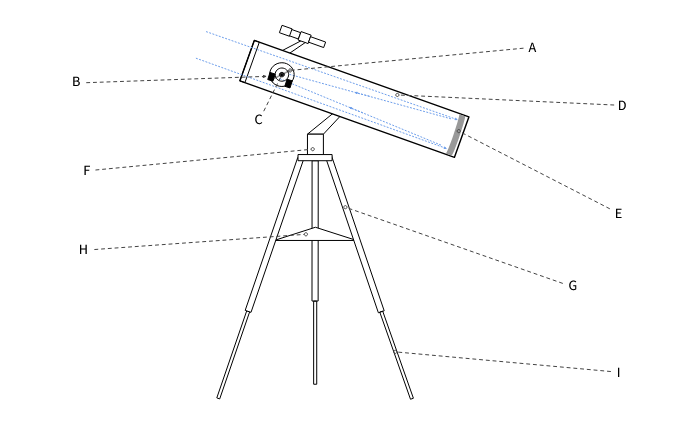
\includegraphics[width=1\textwidth]{images/telescope.png}
          \end{center}
          \begin{center}
              \makebox[5pt]{%
                  \(
                  \begin{array}{ccc}
                      \text{(A) Eyepiece Holder} \hspace{2cm} & \text{(B) Focuser} \hspace{2cm}             & \text{(C) Eyepiece} \hspace{2cm}         \\
                      \text{(D) Telescope Tube} \hspace{2cm}  & \text{(E) Primary Mirror Cell} \hspace{2cm} & \text{(F) Mount} \hspace{2cm}            \\
                      \text{(G) Outer Tripod} \hspace{2cm}    & \text{(H) Accessory Tray} \hspace{2cm}      & \text{(I) Tripod Extension} \hspace{2cm}
                  \end{array}
                  \)
              }
          \end{center}
    \item[\textbf{Problem B}]{
          If the diameter of the sun is 1,400,000km ($1.4\times10^{6}km = 1.4\times10^{6}km\cdot10^{5}\frac{cm}{km} = 1.4\times10^{11}cm$ ) and it is now 22cm, then the ratio of the old diameter to the new diameter is:
          \begin{center}
              \[
                  %   \text{let } 
                  r = \frac{2.2 \times 10^{1}}{1.4 \times 10^{11}} = 1.571428 \times 10^{-10}
              \]

          \end{center}
          At this scale, the distance of the sun to the earth, \begin{center}
              \[
                  \text{1 AU} = 1.496 \times 10^{8} km = 1.496 \times 10^{8}\cdot10^{5}\frac{cm}{km} = 1.496 \times 10^{13}
              \]
              would be equal to,
              \[
                  \text{1 }AU_{scaled} =  1.496 \times 10^{13}cm \cdot 1.571428 \times 10^{-10} = 9.520003\times10^{3}cm = 952.0003cm
              \]
          \end{center}
          \newpage
          The diameter of the earth, originally 12,750km, \[d_{e0} = 1.275\times10^{4}km = 1.275\times10^{4}km\cdot10^{5}\frac{cm}{km} = 1.275\times10^{9}cm\]
          would be equivalent to,
          \begin{center}
              \[
                  d_{e1} = 1.275 \times 10^{9} \cdot 1.571428 \times 10^{-10} = 2.00357172 \times 10^{-1}cm
              \]
          \end{center}}
          The distance from earth to the closest star, 4.25 light years, is
          \begin{center}
              \[
                  4.25 \text{ light years} = 4.25 \times 10^{0} \text{ light years} \cdot 9.46073 \times 10^{12} \frac{km}{\text{light year}} \cdot 10^{5}\frac{cm}{km} = 4.02081 \times 10^{18} cm
              \]

              \[
                  d_{s} = 4.02081 \times 10^{18} cm \cdot 1.571428 \times 10^{-10} = 6.31841380954 \times 10^{8} \text{ cm}
              \]
          \end{center}
    \item[\textbf{Problem C}]{
          \newtheorem*{problem}{Part A}
          \begin{problem}
          Verify that the following equation is valid for the density of a planet given its gravitational acceleration \(g\) and radius \(R\):
          \begin{equation}
              \rho(g, R) = \frac{3}{4 \gamma \pi} \cdot g \cdot \frac{1}{R}
          \end{equation}
          Here, \(\gamma\) is the gravitational constant ($6.674 \times 10^{-11} \mskip\thinmuskip m^3kg^{-1}s^{-2}$), and \(\rho = \frac{m}{V}\) where \(m\) is the planet's mass and \(V\) its volume. Since the volume of a sphere is \(V = \frac{4}{3}\pi R^3\), we can write:

          \begin{equation}
              \frac{m}{\frac{4}{3}\pi R^3} = \frac{3}{4 \gamma \pi} \cdot g \cdot \frac{1}{R}
          \end{equation}
          simplifying gives us:
          \begin{equation}
              \frac{m}{R^3} = \frac{1}{\gamma} \cdot g \cdot \frac{1}{R}
          \end{equation}
          if we tak the invrse of both sides, divide by \(R^2\), and multiply by \(g\) we get:
          \begin{equation}
              g = \frac{\gamma \cdot m}{R^2}
          \end{equation}
          which looks like the equation for gravitational acceleration, thus prooving that the equation is valid.
          \begin{equation}
              g = \frac{G \cdot m}{R^2}
          \end{equation}
          We can also perform dimensional analysis, starting from the simplified equation above:
          \begin{equation}
              \frac{m}{R^2} = \frac{1}{\gamma} \cdot g
          \end{equation}
          substuting the units of \(\gamma\), \(g\), \(R\), and \(m\) gives us:
          \begin{equation}
              \frac{kg}{m^2} = \frac{1}{\frac{m^3}{kg \cdot s^2}} \cdot \frac{m}{s^2}
          \end{equation}
          \begin{equation}
              \frac{kg}{m^2} = \frac{kg \cdot s^2}{m^3} \cdot \frac{m}{s^2}
          \end{equation}
          \begin{equation}
              \frac{kg}{m^2} = \frac{kg}{m^2}
          \end{equation}

          Dimensional analysis proves that the equation is valid.

          \end{problem}
          \newtheorem*{problem2}{Part B}
          \begin{problem2}
              Given the earth's gravitational acceleration \(g = 9.81 \mskip\thinmuskip m/s^2\) and radius \(R = \frac{12750}{2}\mskip\thinmuskip km = 6.375 \times 10^3 \mskip\thinmuskip km\), we can calculate the density of the earth using the equation:
              \begin{equation}
                  \rho(g, R) = \frac{3}{4 \gamma \pi} \cdot g \cdot \frac{1}{R}
              \end{equation}
              Replacing the values of \(g\), \(R\), and \(\gamma\) with units gives us:
              \begin{equation}
                  \rho(9.81 \mskip\thinmuskip m/s^2, 6.375 \times 10^3 \mskip\thinmuskip km) = \frac{3}{4 \cdot 6.674 \times 10^{-11} \mskip\thinmuskip m^3kg^{-1}s^{-2} \cdot \pi} \cdot 9.81 \mskip\thinmuskip m/s^2 \cdot \frac{1}{6.375 \times 10^3 \mskip\thinmuskip km}
              \end{equation}
              Converting \(R\) to meters gives us \(R = 6.375 \times 10^3 \mskip\thinmuskip km = 6.375 \times 10^6 \mskip\thinmuskip m\). Substituting this value into the equation gives us:
              \begin{equation}
                  \rho(9.81 \mskip\thinmuskip m/s^2, 6.375 \times 10^6 \mskip\thinmuskip m) = \frac{3}{4 \cdot 6.674 \times 10^{-11} \mskip\thinmuskip m^3kg^{-1}s^{-2} \cdot \pi} \cdot 9.81 \mskip\thinmuskip m/s^2 \cdot \frac{1}{6.375 \times 10^6 \mskip\thinmuskip m}
              \end{equation}
              Calculating this gives us:
              \begin{equation}
                  \rho(9.81 \mskip\thinmuskip m/s^2, 6.375 \times 10^6 \mskip\thinmuskip m) \approx 5.515 \times 10^{3} kg/m^3
              \end{equation}
          \end{problem2}
          }
    \item[\textbf{Problem D}]{
          \newtheorem*{problem3}{}
          \begin{problem3}
              If we assume a model $a(t) = \lambda \cdot t^\beta$ for the scale factor, then the derivative of the scale factor with respect to time is:
              \begin{equation}
                  \dot{a}(t) = \lambda \cdot \beta \cdot t^{\beta - 1}
              \end{equation}
              Then Hubble parameter would be defined as:
              \begin{equation}
                  H(t) = \frac{\dot{a}(t)}{a(t)} = \frac{\lambda \cdot \beta \cdot t^{\beta - 1}}{\lambda \cdot t^\beta} = \frac{\beta}{t}
              \end{equation}
              The derivative of the Hubble parameter with respect to time is:
              \begin{equation}
                  \dot{H}(t) = \frac{d}{dt}\left(\frac{\beta}{t}\right) = -\frac{\beta}{t^2}
              \end{equation}
              The deacceleration parameter is defined as:
              \begin{equation}
                  q(t) = -\left(1 + \frac{\dot{H}(t)}{H(t)^2}\right) = -\left(1 + \frac{-\beta}{t^2} \cdot \frac{t^2}{\beta^2}\right) = -\left(1 - \frac{1}{\beta}\right)
              \end{equation}
              If we assume that in 2024, the Hubble parameter is \(H(2024) = 72.6 \mskip\thinmuskip km/s/Mpc\), then we can calculate the deacceleration parameter for the age of the universe, which is approximately 13.7 billion years, or \(t = 1.37 \times 10^{10} \mskip\thinmuskip years \cdot 3.1536
              \times 10^{7} \mskip\thinmuskip \frac{s}{years}  = 4.320432 \times 10^{17} \mskip\thinmuskip s\). Calculating $\beta$ gives us:
              \begin{equation}
                  \beta = H(4.320432 \times 10^{17} \mskip\thinmuskip s) \cdot 4.32 \times 10^{17} \mskip\thinmuskip s = 72.6 \mskip\thinmuskip km/s/Mpc \cdot 4.32 \times 10^{17} \mskip\thinmuskip s = 3.1366 \times 10^{19} \mskip\thinmuskip km/Mpc
              \end{equation}
              Substituting this value into the equation for the deacceleration parameter gives us:
              \begin{equation}
                  q(4.320432 \times 10^{17} \mskip\thinmuskip s) = -\left(1 - \frac{1}{3.1366 \times 10^{19}}\right) \approx -1
              \end{equation}

              From this, we can see that the universe is currently accelerating, as the deacceleration parameter is negative. This means that the universe is expanding at an increasing rate.


          \end{problem3}}
    \item[\textbf{Problem E}]{
          A comet is a large object made of ice and dust that orbits the sun. The bright tail forms as the comet approaches the sun, causing the ice to vaporize and release gas and dust particles.
          }

\end{enumerate}

\end{document}